\documentclass[12pt]{article}
\usepackage{amsmath}
\usepackage{multirow}
\usepackage{enumerate}
\usepackage{graphicx}
\usepackage{changepage}
\usepackage[all]{xy}
\usepackage{tikz}
\usetikzlibrary{shapes}

\setlength{\voffset}{-3cm}
\setlength{\hoffset}{-2cm}
\setlength{\parindent}{0cm}
\setlength{\textheight}{27cm}
\setlength{\textwidth}{17cm}


\begin{document}

\quad\\[2cm]

\begin{center}
{\Huge Statistics for Computing MA4413\\[0.8cm]
Midterm Examination 2\\[1cm]
{\bf Type B}}\\[2cm]
\end{center}

\begin{itemize}\itemsep0.6cm
\item Do not turn over the page until instructed to do so.
\item Rough work pages are provided within.
\item Useful formulae and statistical tables are provided at the back.
\item {\bf Enter your answers (using an ``X'') in the table on the last page.}
\item There are 15 questions in total: each correct answer = 1\% with {\bf no negative marks}.
\item For each question, only \emph{one} answer is correct.
\item Scientific calculators approved by the University of Limerick can be used.
\end{itemize}

\newpage
\section*{Questions 1 - 5}


\rule{\linewidth}{1pt}
\quad\\
Let $X \sim \text{Normal}(\mu=15,\sigma=3)$.\\{\footnotesize(Note: answers below are given to two decimal places)}\\[0.2cm]

{\bf Q1} What is the value of $\Pr(X > 18.66)$?\\[0.2cm]
\begin{tabular}{cccc}
{\bf(a)} $0.34$ & {\bf(b)} $0.11$ & {\bf(c)} $0.89$  & {\bf(d)} $0.22$ \\[0.6cm]
\end{tabular}


{\bf Q2} What is the value of $x$ such that $\Pr(X > x) = 0.8$?\\[0.2cm]
\begin{tabular}{cccc}
{\bf(a)} $7.43$  & {\bf(b)} $22.57$ & {\bf(c)} $17.52$ & {\bf(d)} $12.48$   \\[0.6cm]
\end{tabular}

%Let $X_1 \sim \text{Normal}(\mu_1=10,\sigma=4)$ and $X_2 \sim \text{Normal}(\mu_2=8,\sigma=3)$.\\[0.2cm]
%
%{\bf Q10} What is the value of $\Pr(X_1-X_2 < 0)$? {\footnotesize(rounded to 2 decimal places)}\\[0.2cm]
%\begin{tabular}{cccc}
%{\bf(a)} 0.40 & {\bf(b)} 0.34 & {\bf(c)} 0.66 & {\bf(d)} 0.60 \\[0.6cm]
%\end{tabular}


\rule{\linewidth}{1pt}
\quad\\
The voting population of Ireland is approximately 2,800,000. It was of interest to gain insight into the voting intentions of the public prior to an upcoming referendum - more specifically, the \emph{proportion} of voters who intended to vote ``Yes'' was of interest. Therefore, 877 individuals were contacted of which 492 said they would vote ``Yes''.
\\[0.2cm]


{\bf Q3} What is the sample size?\\[0.2cm]
\begin{tabular}{cccc}
{\bf(a)} $877$ & {\bf(b)} $2,800,000$ & {\bf(c)} unknown & {\bf(d)} $492$ \\[0.6cm]
\end{tabular}

{\bf Q4} What is the value of the statistic? \\[0.2cm]
\begin{tabular}{cccc}
{\bf(a)} $\bar x = 492$  & {\bf(b)} $\bar x = 0.56$ & {\bf(c)} $\hat p = 492$ & {\bf(d)} $\hat p = 0.56$ \\[0.6cm]
\end{tabular}


\rule{\linewidth}{1pt}

\quad\\
Consider the following sample of ages of computers in an office block:
\begin{center}
\begin{tabular}{|ccc|}
\hline
&&\\[-0.3cm]
5.3 & 7.8 & 4.9 \\[0.1cm]
\hline
\end{tabular}
\end{center}
{\bf Q5} The 95\% confidence interval for the mean is:\\[0.2cm]
\begin{tabular}{cccc}
{\bf(a)} $[2.096,\,\,9.904]$ & {\bf(b)} $[4.222,\,\,7.778]$ & {\bf(c)} $[3.350,\,\,8.650]$ & {\bf(d)} $[-0.136,\,\,12.136]$ \\[0.6cm]
\end{tabular}

\quad

\rule{\linewidth}{1pt}

\newpage

\section*{Rough Work\\[23cm]}
\section*{\hspace{8cm}$\boxed{\text{Next page: Questions 6 - 10}}$}

\newpage


\section*{Questions 6 - 10}


\rule{\linewidth}{1pt}
\quad

On average, flaws arise on a fibre optic cable at a rate of $0.5$ per km (kilometer) according to a Poisson distribution.\\[0.2cm]

{\bf Q6} What is the probability that there are \emph{less than} 3 flaws in 6~km of this cable? \\[0.2cm]
\begin{tabular}{cccc}
{\bf(a)} $0.3734$ & {\bf(b)} $0.6472$ & {\bf(c)} $0.4232$ & {\bf(d)} $0.2240$ \\[0.6cm]
\end{tabular}

{\bf Q7} What is the standard deviation for the number of flaws in 80 km of cable?\\[0.2cm]
\begin{tabular}{cccc}
{\bf(a)} $0.158$  & {\bf(b)} $0.025$ & {\bf(c)} $40$  & {\bf(d)} $6.325$ \\[0.6cm]
\end{tabular}


\rule{\linewidth}{1pt}
\quad\\
{\bf Q8} Identify the statement that is \emph{true} (note: only one is true).\\[0.2cm]
%{\footnotesize(answer is given to two decimal places)}\\[0.2cm]
\begin{tabular}{c@{\,\,\,}llll}
{\bf(a)} & We always know the value of the parameter. \\[0.2cm]
{\bf(b)} & The standard error tends to increase as the sample size increases. \\[0.2cm]
{\bf(c)} & A 95\% confidence interval is wider than a 90\% confidence interval. \\[0.2cm]
{\bf(d)} & The population mean varies from sample to sample. \\[0.6cm]
\end{tabular}


\rule{\linewidth}{1pt}
\quad\\
Assume that the time taken to complete this exam has an exponential distribution with parameter $\lambda = 0.025$, i.e., $T \sim \text{Exponential}(\lambda=0.025)$.\\[0.3cm]
{\bf Q9} What is the value of the probability $\Pr(20 < T < 40)$? \\[0.2cm]
\begin{tabular}{cccc}
{\bf(a)} 0.6667 & {\bf(b)} 0.2387 & {\bf(c)} 0.2231 & {\bf(d)} 0.5\\[0.6cm]
\end{tabular}

{\bf Q10} A sample of 64 students are selected; let $\,\overline{\!T}$ be the \emph{sample mean}, i.e., the mean calculated for this sample of students. What is the value of the probability $\Pr(\,\overline{\!T} > 48)$? \\[0.2cm]
\begin{tabular}{cccc}
{\bf(a)} $0.0548$ & {\bf(b)} $ 0.0047$ & {\bf(c)} $0.1446$  & {\bf(d)} $0.3012$ \\[0.6cm]
\end{tabular}


\rule{\linewidth}{1pt}

\newpage

\section*{Rough Work\\[23cm]}
\section*{\hspace{8cm}$\boxed{\text{Next page: Questions 11 - 15}}$}

\newpage

\section*{Questions 11 - 15}

\rule{\linewidth}{1pt}
\quad\\
Consider an $M/M/1$ system where customers arrive at a rate of 1.5/min and the average time spent in the \emph{service node} is 15 seconds.\\[0.2cm]

{\bf Q11} What is the utilisation factor?\\[0.2cm]
\begin{tabular}{cccc}
{\bf(a)} $0.375$ & {\bf(b)} $4.00$ & {\bf(c)} $0.250$ & {\bf(d)} $2.667$ \\[0.6cm]
\end{tabular}

{\bf Q12} On average, how many customers are in the \emph{whole system}?\\[0.2cm]
\begin{tabular}{cccc}
{\bf(a)} $0.4$ & {\bf(b)} $1.6$ & {\bf(c)} $4.0$ & {\bf(d)} $0.6$ \\[0.6cm]
\end{tabular}

\rule{\linewidth}{1pt}
\quad\\
A manufacturer wants to compare two designs of CPU in terms of their typical operating temperature (degrees Celsius). Two large samples are selected and the results are as follows:
\begin{small}
\begin{center}
\begin{tabular}{|c|c|c|}
\hline
&&\\[-0.3cm]
& Design 1 & Design 2 \\
\hline
&&\\[-0.2cm]
sample size      & 40 & 50 \\[0.2cm]
mean   & 38.7 $^\circ$C & 32.1 $^\circ$C \\[0.2cm]
variance &  3.0 $^\circ$C$^2$ & 8.0 $^\circ$C$^2$ \\[0.2cm]
\hline
\multicolumn{3}{c}{}
\end{tabular}
\end{center}
\end{small}


{\bf Q13} The 84\% confidence interval for $\mu_1-\mu_2$ is:\\[0.2cm]
%{\footnotesize(hint: use tables)}\\[0.2cm]
\begin{tabular}{cccc}
{\bf(a)} $[6.12,\,\,7.08]$ & {\bf(b)} $[4.87,\,\,8.33]$ & {\bf(c)} $[5.92,\,\,7.28]$ & {\bf(d)} $[5.65,\,\,7.55]$ \\[0.6cm]
\end{tabular}


{\bf Q14} What type of data was collected on each CPU? \\[0.2cm]
%{\footnotesize(hint: cannot use tables)}\\[0.2cm]
\begin{tabular}{cccc}
{\bf(a)} numeric continuous & {\bf(b)} numeric discrete  & {\bf(c)} mean data  & {\bf(d)} categorical \\[0.6cm]
\end{tabular}





\rule{\linewidth}{1pt}
\quad\\
Patients with a particular disease can be treated using treatment A or B. It was of interest to estimate the \emph{difference} in proportions of patients cured of the disease under the two treatment regimes, i.e., $p_A - p_B$. Hence, a sample of data was collected and the following 99\% confidence interval for $p_A - p_B$ was calculated: $[0.12,\,0.26]$.\\[0.2cm]

{\bf Q15} What can we say based on the above confidence interval?\\
(note: a bigger cured proportion is better)\\[0.2cm]
\begin{tabular}{c@{\,\,\,}llll}
{\bf(a)} & The evidence suggests that treatment A is better.\\[0.2cm]
{\bf(b)} & The evidence suggests that treatment B is better. \\[0.2cm]
{\bf(c)} & Without any doubt, treatment A is better. \\[0.2cm]
{\bf(d)} & There is no evidence of a difference in treatments. \\[0.6cm]
\end{tabular}


\rule{\linewidth}{1pt}







\newpage

\section*{Rough Work\\[23cm]}
\section*{\hspace{2cm}$\boxed{\text{Don't forget to enter your answers on the last page!}}$}

\newpage


\section*{Useful Formulae: Page 1\\[0.3cm]}
{\bf Numerical Summaries:}\\[-0.8cm]
\begin{align*}
\bullet\quad \bar x &= \frac{\sum\,x_i}{n}\\[0.6cm]
\bullet\quad s^2 &= \frac{\sum\,x_i^2 - n\,\bar x^2}{n-1}\\
\end{align*}
{\bf Probability:}\\[-0.8cm]
\begin{align*}
\bullet\quad \Pr(A^c) &= 1 - \Pr(A) \\[1cm]
\bullet\quad \Pr(A \cup B) &= \Pr(A) + \Pr(B) - \Pr(A \cap B)\\[0.6cm]
\bullet\quad \Pr(E_1 \cup E_2 \cup \cdots \cup E_k) &= \Pr(E_1) + \Pr(E_2) + \cdots + \Pr(E_k) \text{\quad{\footnotesize(if mutually exclusive)}}\\[1cm]
\bullet\quad \Pr(A \cap B) &= \Pr(A) \, \Pr(B \, | \, A) = \Pr(B) \, \Pr(A \, | \, B) \\[0.6cm]
\bullet\quad \Pr(E_1 \cap E_2 \cap \cdots \cap E_k) &= \Pr(E_1) \, \Pr(E_2) \, \cdots \, \Pr(E_k) \text{\quad{\footnotesize(if independent)}}\\[1cm]
\bullet\quad \Pr(A\,|\,B) &= \frac{\Pr(A \cap B)}{\Pr(B)} = \frac{\Pr(A) \,\Pr(B\,|\,A)}{\Pr(B)}\\[1cm]
\bullet\quad \text{If $E_1,\ldots, E_k$} & \,\, \text{are mutually exclusive \& exhaustive}\\[0.1cm]
\Rightarrow \Pr(B) &= \Pr(B \cap E_1) + \Pr(B \cap E_2) + \cdots + \Pr(B \cap E_k) \\[0.2cm]
&= \Pr(E_1) \, \Pr(B\,|\,E_1) + \Pr(E_2) \, \Pr(B\,|\,E_2) + \cdots + \Pr(E_k) \, \Pr(B\,|\,E_k)\\
\end{align*}
{\bf Distributions:}\\[-0.8cm]
\begin{center}
\begin{tabular}{|c@{\qquad}|c@{\qquad}|c@{\qquad}|}
\hline
&&\\[-0.3cm]
$\bullet\quad X \sim \text{Poisson}(\lambda)$ & $\bullet\quad T \sim \text{Exponential}(\lambda)$ & $\bullet\quad X \sim \text{Normal}(\mu,\sigma)$ \\[0.6cm]
${\displaystyle\bullet\quad \Pr(X=x) = \frac{\lambda^x}{x\,!}\,\,e^{-\lambda}}$ & $\bullet\quad \Pr(T>t) = e^{-\lambda\,t}$ & ${\displaystyle\bullet\quad \Pr(X>x) = \Pr\left(Z > \frac{x-\mu}{\sigma}\right)}$\\[0.8cm]
$\bullet\quad x \in \{0,1,2,\ldots,\infty\}$ & $\bullet\quad t \in [0,\,\infty)$ & $\bullet\quad x \in (-\infty,\,\infty)$ \\[0.8cm]
$\bullet\quad E(X) = \lambda$ & ${\displaystyle\bullet\quad E(T) = \frac{1}{\lambda}}$ & $\bullet\quad E(X) = \mu$ \\[0.8cm]
$\bullet\quad Var(X) = \lambda$ & ${\displaystyle\bullet\quad Var(T) = \frac{1}{\lambda^2}}$ & $\bullet\quad Var(X) = \sigma^2$ \\[0.4cm]
\hline
\end{tabular}
\end{center}


\newpage

\section*{Useful Formulae: Page 2\\[0.3cm]}
{\bf Queueing Theory:}\\[-0.8cm]
\begin{align*}
\bullet\quad E(N) &= \lambda_a\,E(T)\\[0.6cm]
\bullet\quad \rho &= \frac{\lambda_a}{\lambda_s}\\[0.6cm]
\xymatrixcolsep{0.5cm}
\bullet\quad M/M/1 \text{ System:} \quad & \xymatrix{\lambda_a \ar@{->}[r] & \hspace{-0.1cm}
{\begin{tabular}{@{}c|@{}c|@{}c|@{}c|@{}c|@{}c}
\cline{1-5}
&&&& &
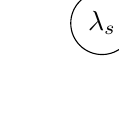
\begin{tikzpicture}[baseline=(char.base)]
\node(char)[draw,shape=circle]{$\lambda_s$};
\end{tikzpicture}\\
\cline{1-5}
\end{tabular}} \hspace{-0.3cm}\ar@{->}[r] &  \lambda_a} \\[0.6cm]
&\Rightarrow \,\, T \sim \text{Exponential}(\lambda_s-\lambda_a)\\[0.1cm]
{\footnotesize(\text{where $T$}} & {\footnotesize\text{ is the total time in the system)}}\\
\end{align*}

{\bf Normal Distribution:}\\[-0.8cm]
\begin{align*}
\bullet\quad \Pr(Z < -z) &= \Pr(Z > z) \\[0.6cm]
\bullet\quad \Pr(Z > -z) &= \Pr(Z < z) = 1 -\Pr(Z>z) \\[0.6cm]
\bullet\quad \Pr(X > x) &= \Pr\left(Z> \frac{x-\mu}{\sigma}\right)\\[0.6cm]
\bullet\quad (1-\alpha)100\% \text{ of the Normal}(\mu,\sigma) & \text{ distribution lies in } \mu \pm z_{\,\alpha/2}\,\,\sigma \\[1cm]
\bullet\quad \text{If} \,\,  X_1 \sim \text{Normal}(\mu_1,\sigma_1) \,\,  & \text{ and } \,\, X_2 \sim \text{Normal}(\mu_2,\sigma_2) \\[0.4cm]
\Rightarrow \quad  \text{ Sum: } \quad  X_1 + X_2 &\sim \text{Normal}\left(\mu_1+\mu_2,\,\sqrt{\sigma_1^2+\sigma_2^2}\,\right) \\[0.4cm]
\Rightarrow \quad  \text{ Difference: } \quad   X_1 - X_2 &\sim \text{Normal}\left(\mu_1-\mu_2,\,\sqrt{\sigma_1^2+\sigma_2^2}\,\right) \\[1cm]
\bullet\quad \text{For} \,\,  X_1,\ldots,X_n \sim \text{any distribution} & \text{ with } \mu = E(X) \text{ and } \sigma = Sd(X) = \sqrt{Var(X)}\\[0.4cm]
\Rightarrow \quad  \text{ Sample mean: } \quad  \,\overline{\!X} &\sim \text{Normal}\left(\mu,\,\frac{\sigma}{\sqrt{n}}\,\right) \quad \text{ if } n > 30
\end{align*}

\newpage


\section*{Useful Formulae: Page 3\\[0.3cm]}
{\bf Confidence Intervals:}\\[-0.8cm]
\begin{align*}
\bullet\quad \text{Large sample:} \qquad \text{statistic } &\pm\,\, z_{\,\alpha/2}\,\times\,\text{standard error} \\[0.6cm]
\bullet\quad \text{Small sample:} \qquad \text{statistic } &\pm\,\, t_{\,\nu,\,\alpha/2}\,\times\,\text{standard error}
\end{align*}
\begin{center}
\begin{tabular}{|c|c|c|c|c|}
\hline
&&&&\\[-0.1cm]
Parameter & Statistic & Standard Error & Samples & D. of. F. \\[0.3cm]
\hline
&&&&\\[-0.1cm]
$\mu$ & $\bar x$ & ${\displaystyle\frac{s}{\sqrt{n}}}$  & large / small & $\nu = n - 1$ \\[0.5cm]
\hline
&&&&\\[-0.1cm]
$p$ & $\hat p$ & \multirow{1}{*}{${\displaystyle\sqrt{\frac{\hat p\,(1-\hat p)}{n}}}$} & large & n/a \\[0.7cm]
\hline
&&&&\\[-0.1cm]
$\mu_1-\mu_2$ & $\bar x_1 - \bar x_2$ & \multirow{3}{*}{${\displaystyle\sqrt{\frac{s_1^2}{n_1}+\frac{s_2^2}{n_2}}}$} & large / small & ${\displaystyle \nu = \frac{(a+b)^2}{\frac{a^2}{n_1-1}+\frac{b^2}{n_2-1}}}$ \\[0.8cm]
&&&& ${\displaystyle a=\frac{s_1^2}{n_1}, \,\,\, b=\frac{s_2^2}{n_2}}$ \\[0.5cm]
\cline{3-5}
&&&&\\[-0.1cm]
&  & ${\displaystyle\sqrt{\frac{s_p^2}{n_1}+\frac{s_p^2}{n_2}}}$ & small & $\nu = n_1+n_2-2$ \\[0.5cm]
&&&& assuming \\[-0.2cm]
&& where\,\, ${\displaystyle s_p^2 = \frac{(n_1-1)\,s_1^2+(n_2-1)\,s_2^2}{n_1+n_2-2}}$  && $\sigma_1^2 = \sigma_2^2$ \\[0.5cm]
\hline
&&&&\\[-0.1cm]
$p_1-p_2$ & $\hat p_1 - \hat p_2$ & \multirow{2}{*}{${\displaystyle\sqrt{\frac{\hat p_1 \, (1-\hat p_1)}{n_1}+\frac{\hat p_2 \, (1-\hat p_2)}{n_2}}}$} & large & n/a\\[0.9cm]
\hline
\multicolumn{5}{c}{}\\[0.5cm]
\end{tabular}
\end{center}
\begin{align*}
\bullet\quad F &= \frac{\text{larger variance}}{\text{smaller variance}} = \frac{s_{\text{larger}}^2}{s_{\text{smaller}}^2} \\[0.3cm]
 & \nu_1 = \text{top sample size} - 1\\[0.1cm]
  & \nu_2 = \text{bottom sample size} - 1
\end{align*}



\newpage


\begin{adjustwidth}{-1cm}{0cm}
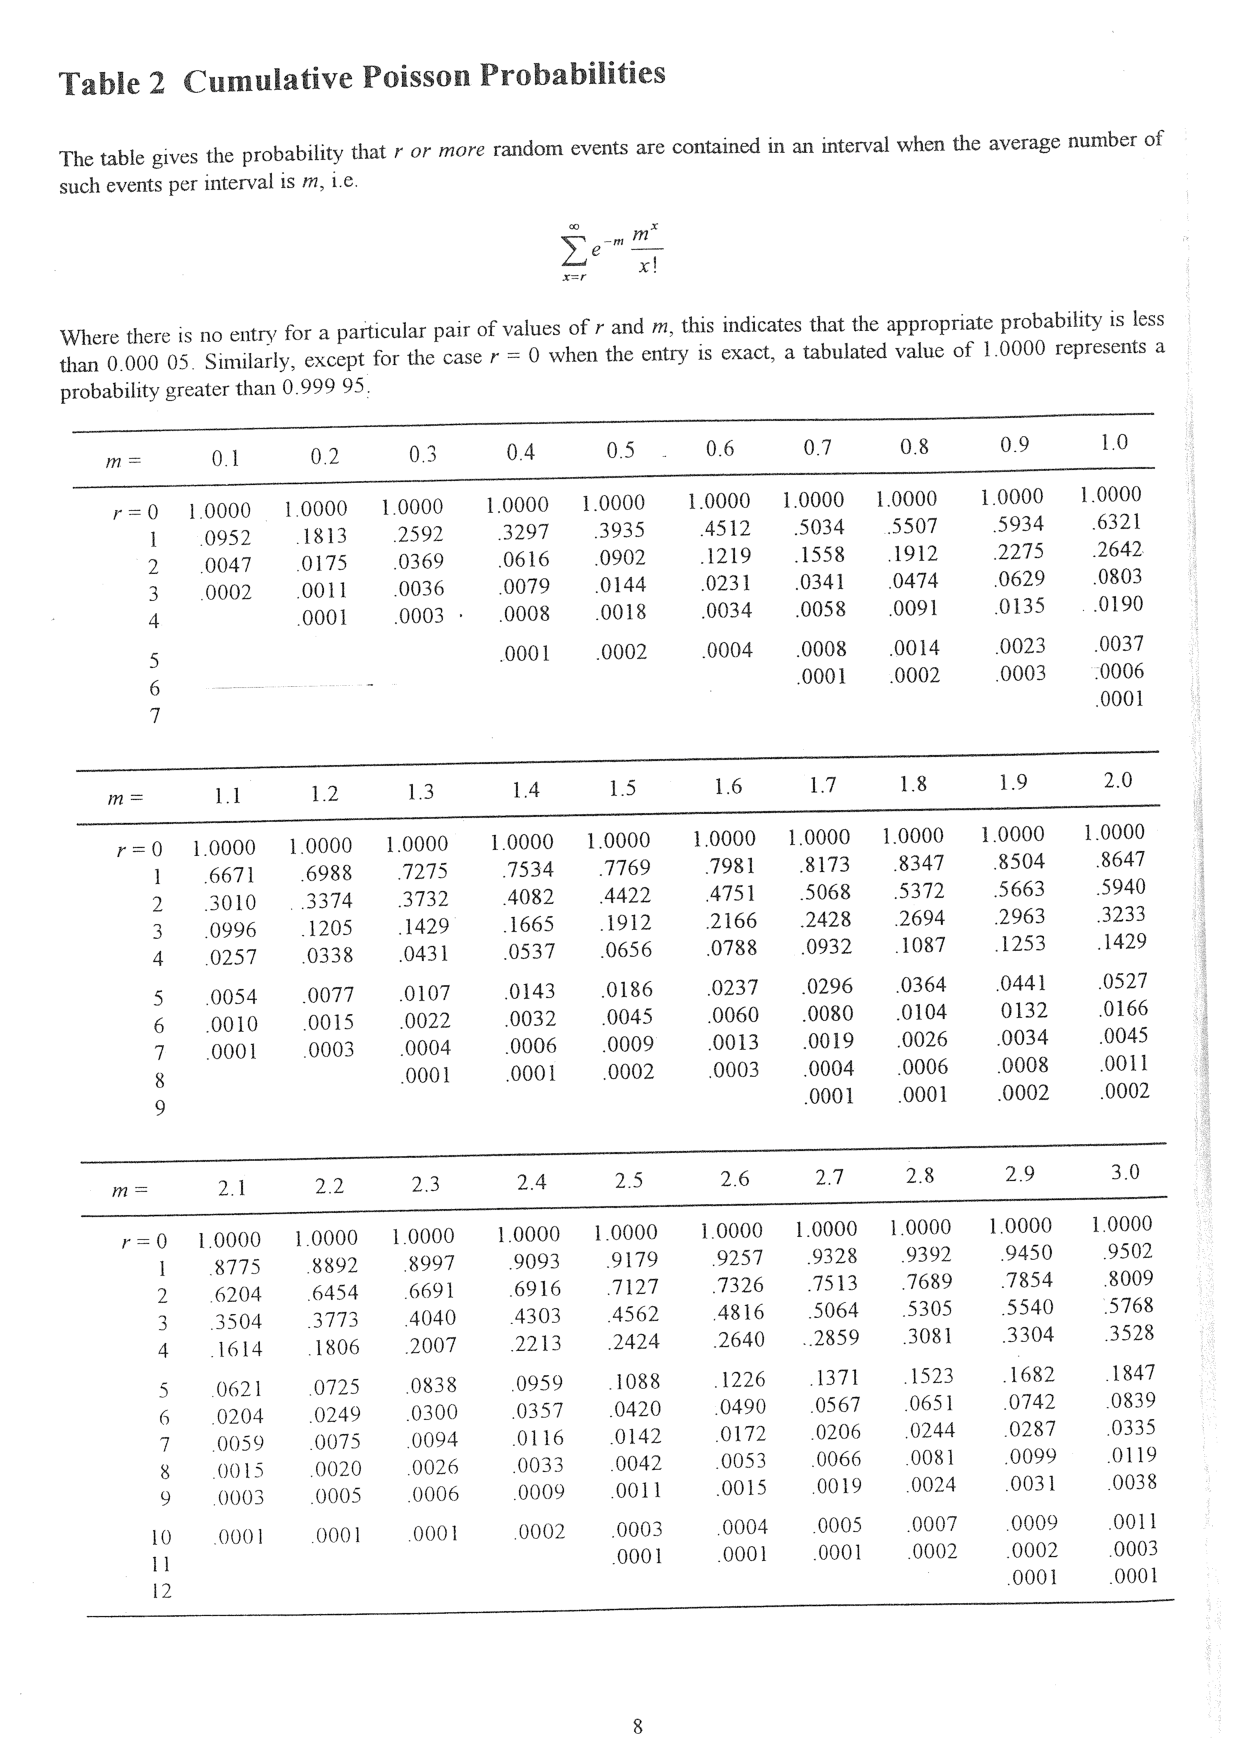
\includegraphics[width=1.1\textwidth, trim = 1cm 1cm 1cm 1cm, clip]{mdpois1}
\end{adjustwidth}

\newpage

\begin{adjustwidth}{-1cm}{0cm}
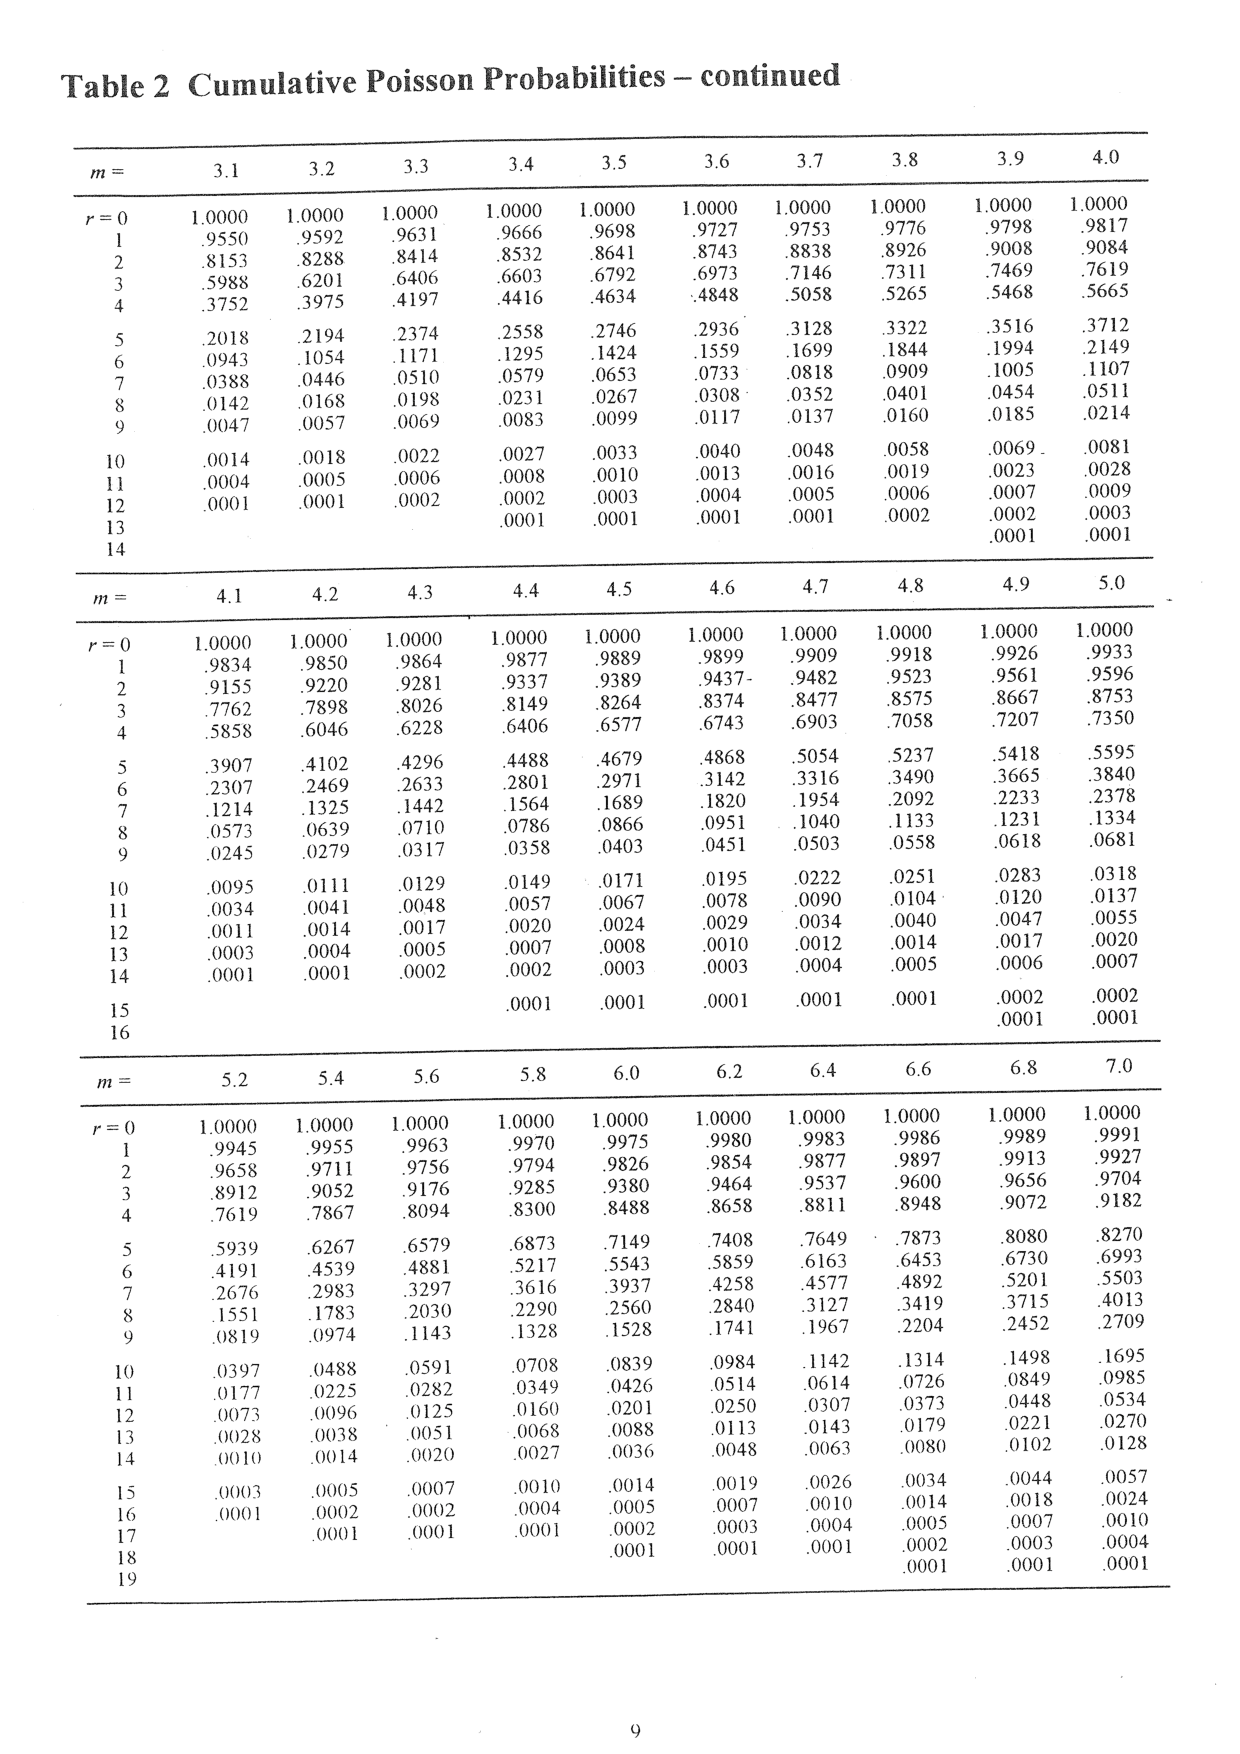
\includegraphics[width=1.1\textwidth, trim = 1cm 1cm 1cm 1cm, clip]{mdpois2}
\end{adjustwidth}

\newpage

\begin{adjustwidth}{-1cm}{0cm}
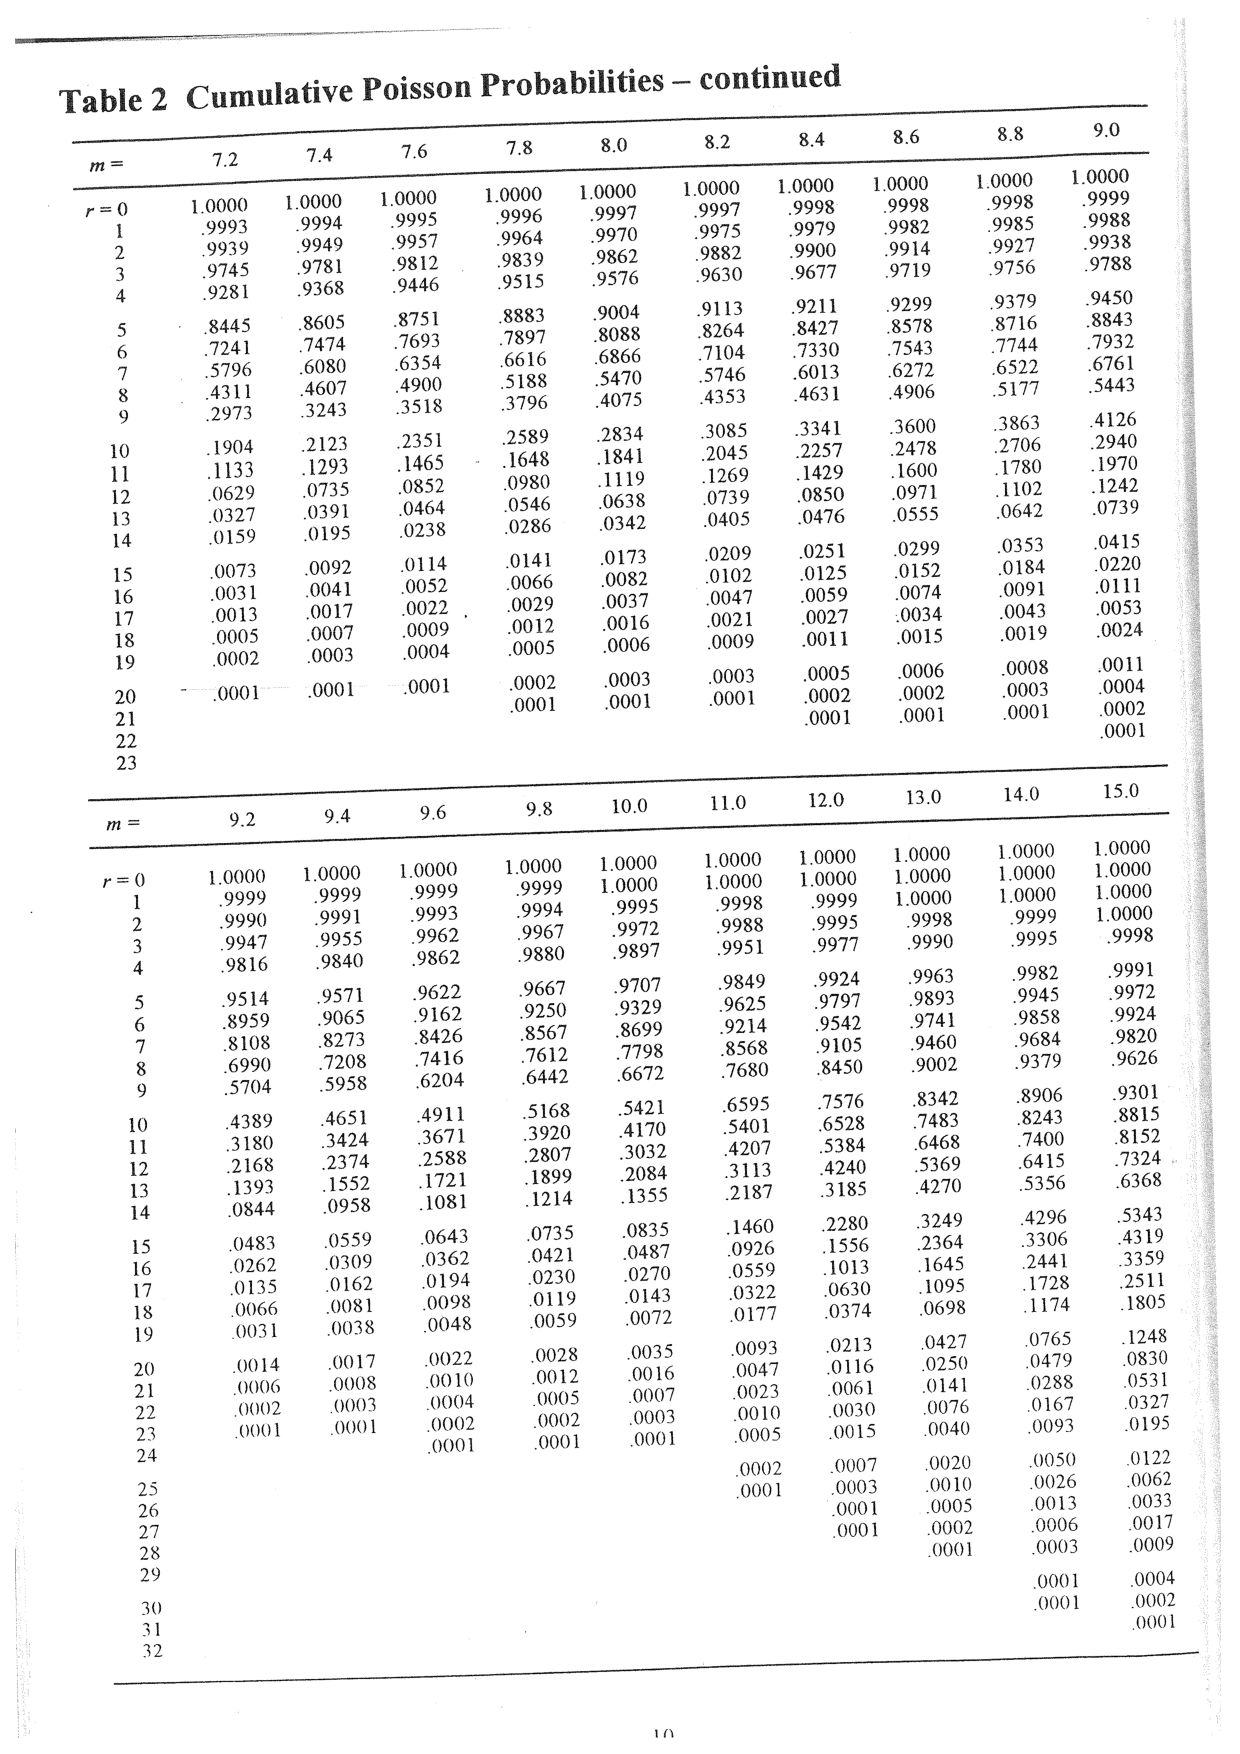
\includegraphics[width=1.1\textwidth, trim = 1cm 1cm 1cm 1cm, clip]{mdpois3}
\end{adjustwidth}

\newpage


\begin{adjustwidth}{-1cm}{0cm}
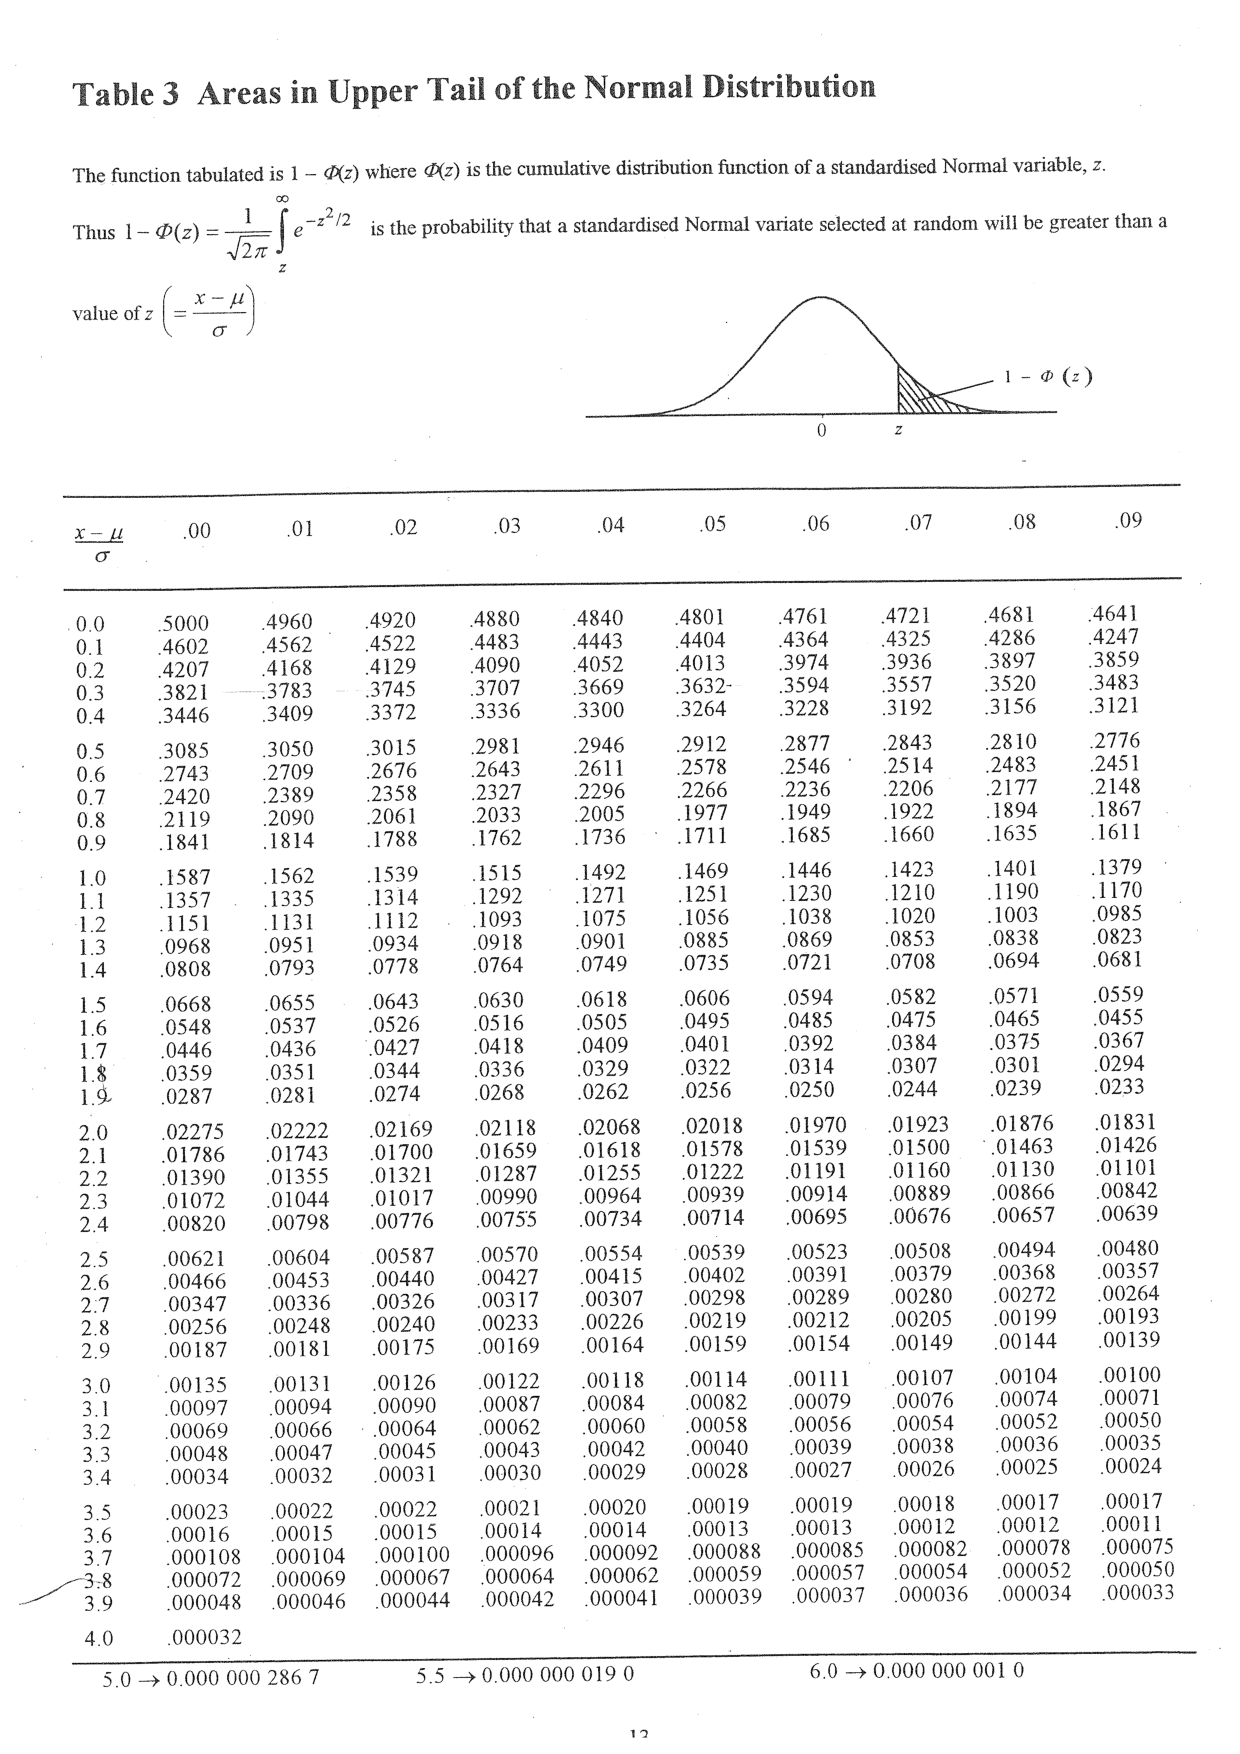
\includegraphics[width=1.1\textwidth, trim = 1cm 1cm 1cm 1cm, clip]{mdnorm}
\end{adjustwidth}

\newpage


\begin{adjustwidth}{-1cm}{0cm}
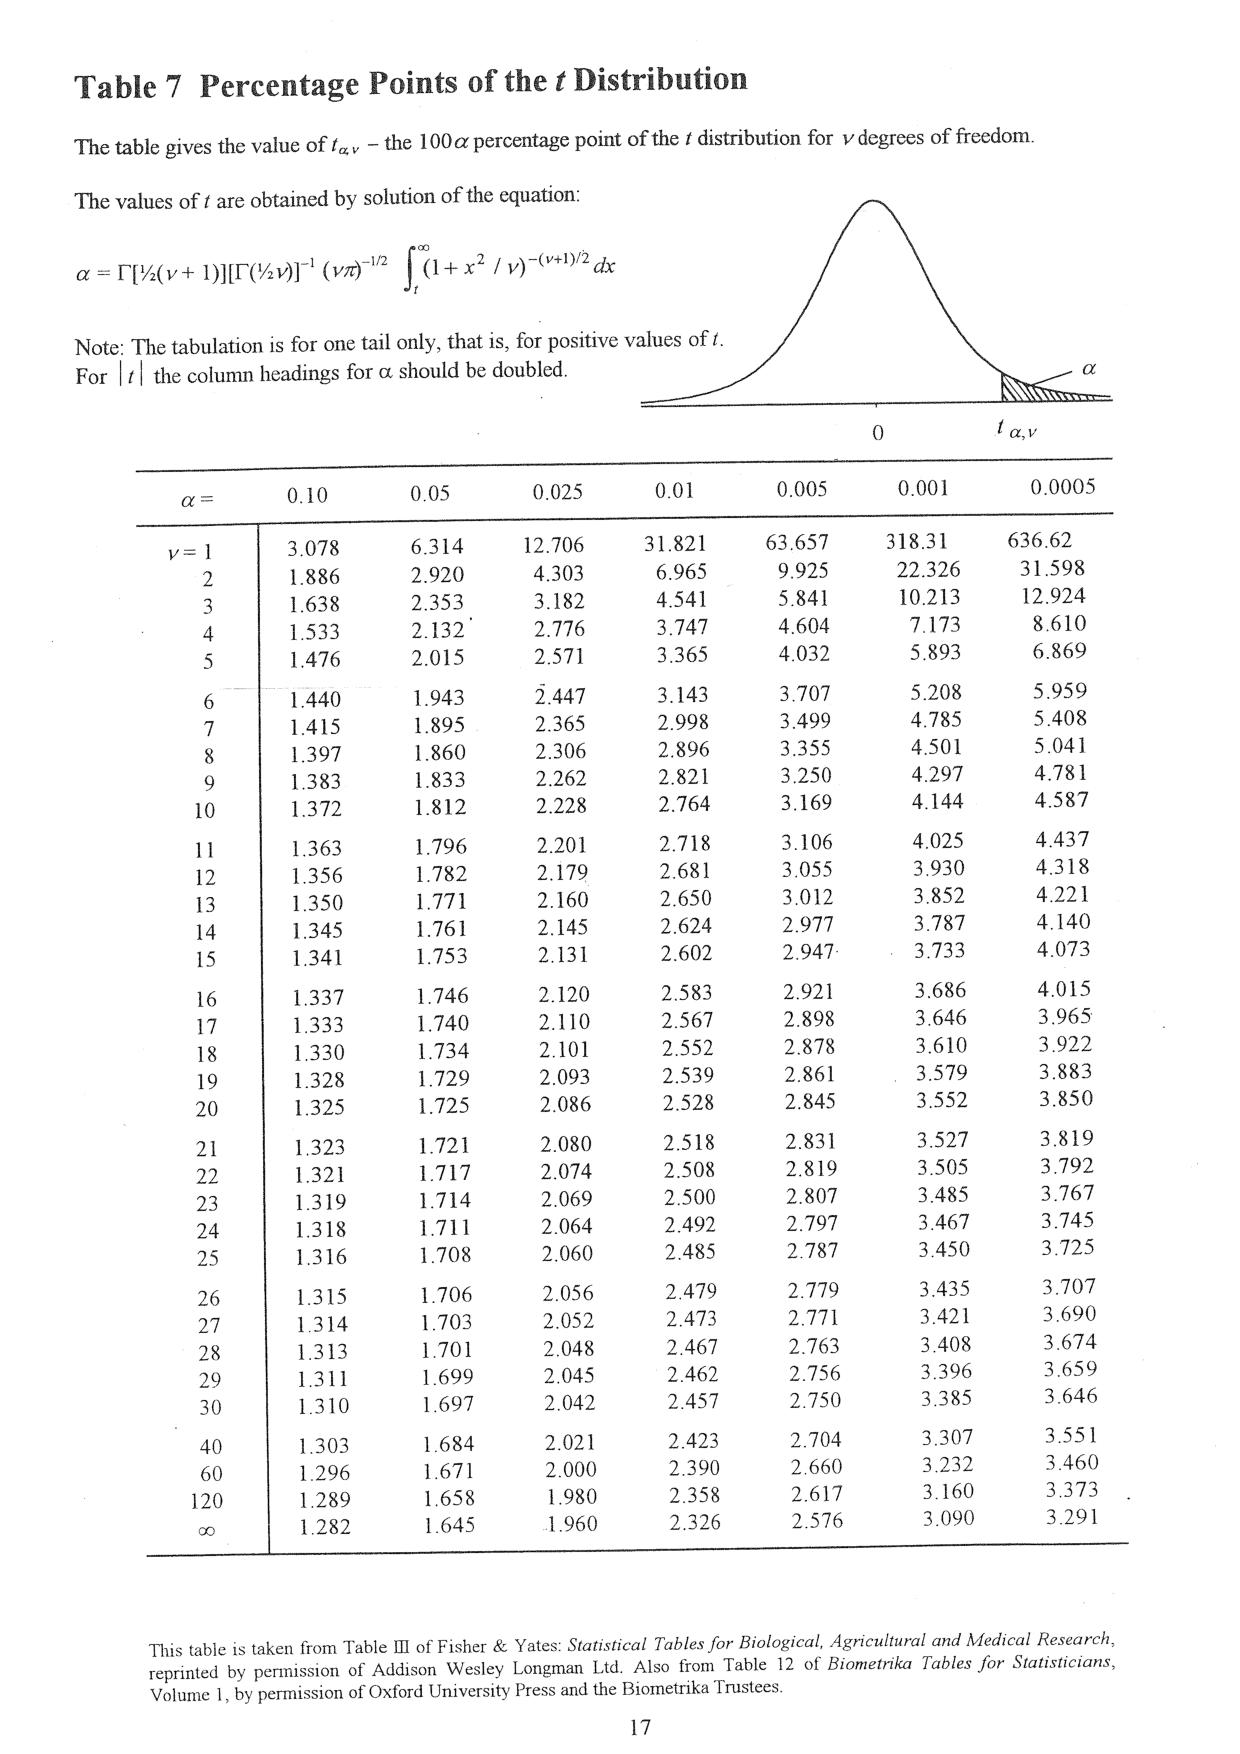
\includegraphics[width=1.1\textwidth, trim = 1cm 1cm 1cm 1cm, clip]{mdt}
\end{adjustwidth}

\newpage



\begin{adjustwidth}{-1cm}{0cm}
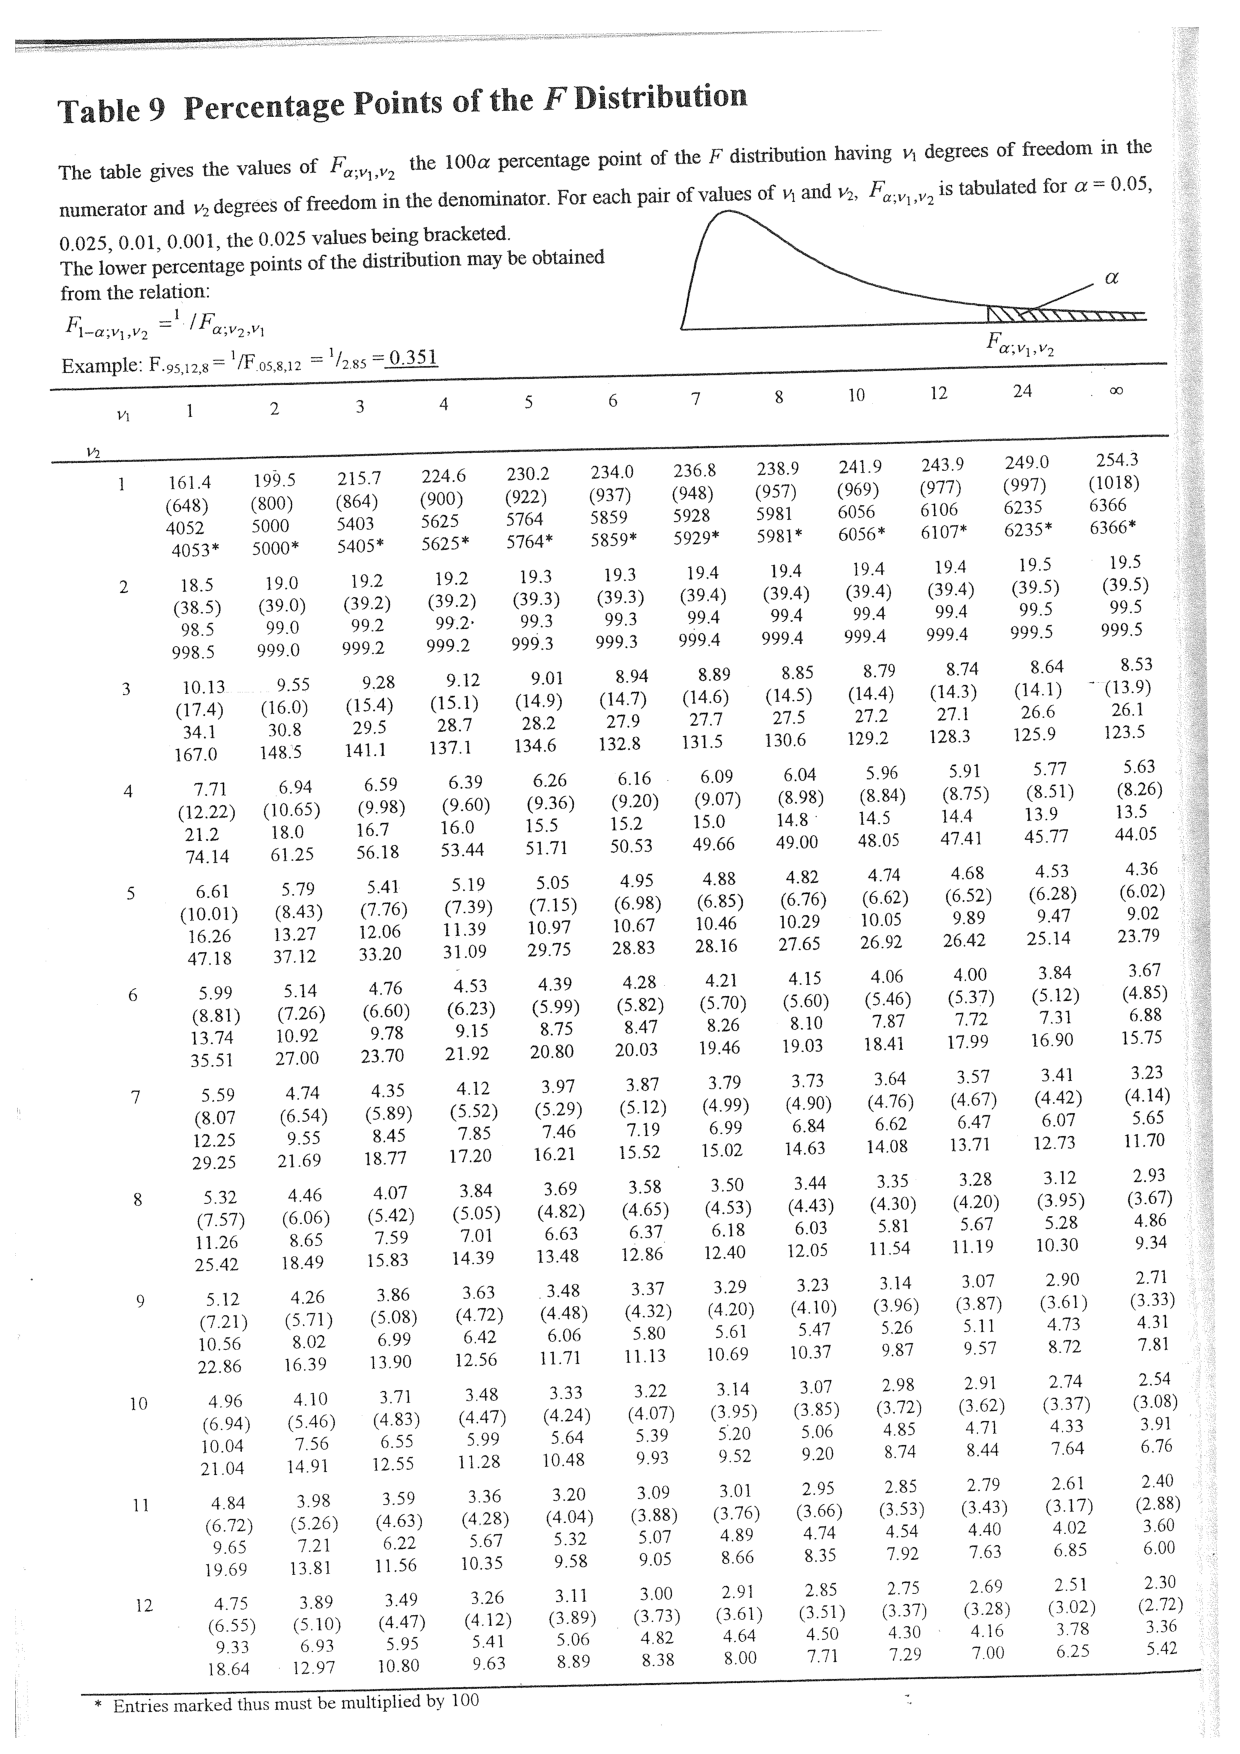
\includegraphics[width=1.1\textwidth, trim = 1cm 0.7cm 1cm 1cm, clip]{mdF}
\end{adjustwidth}

\newpage
\quad
\newpage

\section*{Answer Sheet\\[0.3cm]}

\subsection*{Name:\quad\underline{\hspace{11.45cm}}\\[0.3cm]}
\subsection*{ID Number:\quad\underline{\hspace{10cm}}\\[0.5cm]}

Enter your answers with an ``X' in the table below.\\[0.3cm]
Do not enter the ``X'' until you have made your \emph{final decision} to avoid scribbling out.\\[0.3cm]
\begin{large}
\begin{center}
\begin{tabular}{|c|c|c|c|c|}
\hline
&&&&\\[-0.4cm]
 & A & B & C & D \\
\hline
&&&&\\[-0.4cm]
Q1 &&&& \\
\hline
&&&&\\[-0.4cm]
Q2 &&&& \\
\hline
&&&&\\[-0.4cm]
Q3 &&&& \\
\hline
&&&&\\[-0.4cm]
Q4 &&&& \\
\hline
&&&&\\[-0.4cm]
Q5 &&&& \\
\hline
\multicolumn{5}{c}{}\\[-0.3cm]
\hline
&&&&\\[-0.4cm]
Q6 &&&& \\
\hline
&&&&\\[-0.4cm]
Q7 &&&& \\
\hline
&&&&\\[-0.4cm]
Q8 &&&& \\
\hline
&&&&\\[-0.4cm]
Q9 &&&& \\
\hline
&&&&\\[-0.4cm]
Q10 &&&& \\
\hline
\multicolumn{5}{c}{}\\[-0.3cm]
\hline
&&&&\\[-0.4cm]
Q11 &&&& \\
\hline
&&&&\\[-0.4cm]
Q12 &&&& \\
\hline
&&&&\\[-0.4cm]
Q13 &&&& \\
\hline
&&&&\\[-0.4cm]
Q14 &&&& \\
\hline
&&&&\\[-0.4cm]
Q15 &&&& \\
\hline
\end{tabular}
\end{center}
\end{large}


\end{document} 